

\section{Physikalische Grundlagen}

\subsection{Photometrie}

Die Radiantenergie $Q$ ist die Lichtenergie. Sie wird durch einen Strom von Photonen erzeugt. Die Energie eines Photons ist 
durch $E=h \cdot f$ geben, wobei $h$ das konstante Planksche Wirkungsquantum und $f$ die Frequenz der Welle ist (Welle-Teilchen Dualismus).  

 \begin{figure}[H]
    \centering
    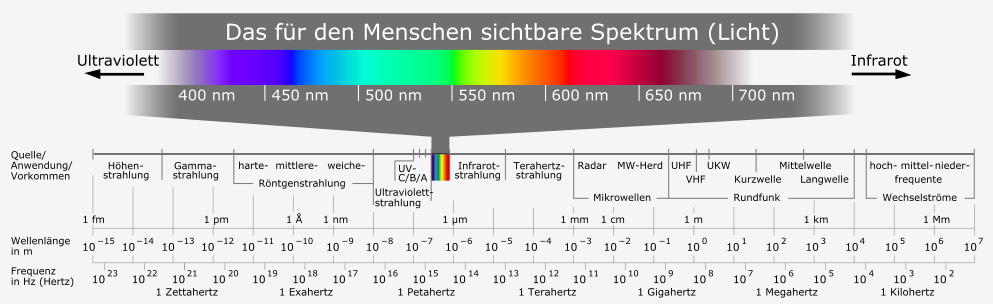
\includegraphics[width=1.0\textwidth]{images/Electromagnetic_spectrum_c.png}
    \caption{Spektrum}
    \label{fig:cray}
\end{figure}


 \begin{figure}[H]
    \centering
    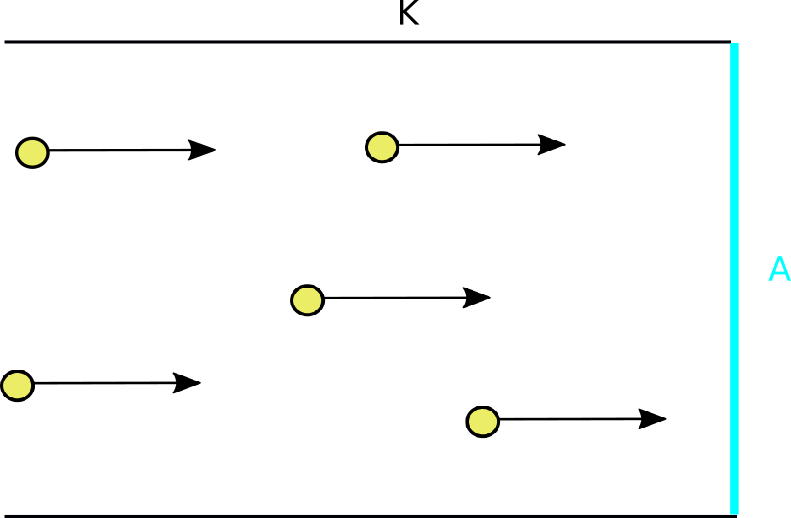
\includegraphics[width=0.75\textwidth]{images/Partikelstrom.png}
    \caption{Partikelstrom in einem Kanal}
    \label{fig:cray}
\end{figure}
Durch einen Kanal $K$ bewegen  sich Teilchen mit gleichförmiger Geschwindigkeit $L$ (Lichtgeschwindigkeit)  und  Dichte $\eta$.
Die Anzahl der Teilchen, die die Fläche $A$ bezüglich eines Zeitintervalles $[0,t]$ passieren, ist gegeben durch
\begin{align}
& D_A([0,t]) := \eta * ||L||  *   \text{Flächeninhalt}(A) *   t 
\end{align}

 Betrachtet man die allgemeinere Situation eines Flächenstückes $B$  in einem Teilchenstorm $L$, so ist die Anzahl gegeben durch 
\begin{align}
D_B([0,t]) := \eta * ||L||  * \cos(\alpha) *  \text{Flächeninhalt} (B) * t
 \end{align}
\begin{figure}[H]
    \centering
    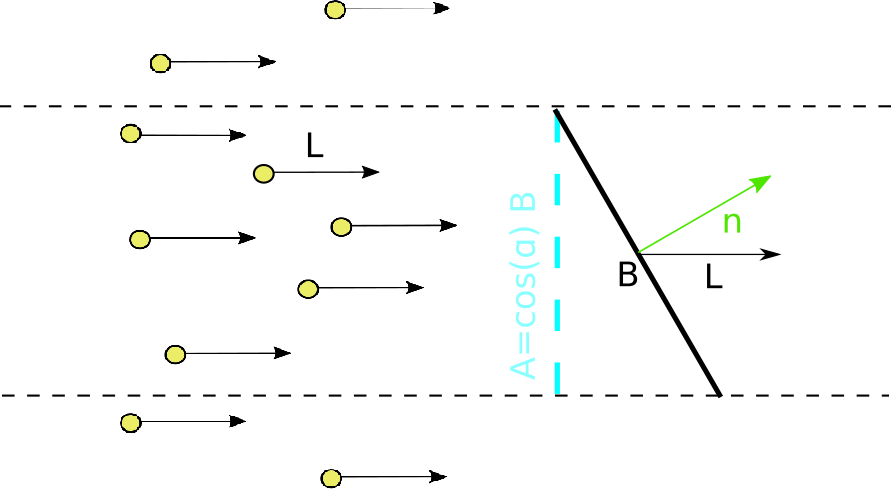
\includegraphics[width=1.0\textwidth]{images/Strahldichte.png}
    \caption{Partikelstrom}
    \label{fig:cray}
\end{figure}
Bezeichnen wir mit $L(B) = \frac{d}{dt \cdot \cos(\theta)}D_B([0,t]) = \eta * ||L||  *  \text{Flächeninhalt} (B)$, so erhalten wir die   Strahldichte als Grenzwert
\begin{align*}
L(x, n):= \lim_{B -> x} L(B)
 \end{align*}
bei dem die Fläche $B$  zu einem Punkt $x$ zusammengezogen wird.  Die Strahlungsleistung aus einer Richtung $\theta$  am Punkt $x$ berechnet sich demnach durch $I(x, \theta) = L(x, \theta) \cdot \cos(\theta)$, was auch als Lambertsches Cosinusgesetz bezeichnet wird.

Angewendet  auf Flächen erhalten wir das  photometrische Grundgesetzt. Es beschreibt die Strahlungleistung, die von einem  Flächenelement auf ein anderes  Flächenelement übertragen wird.

   \begin{figure}[H] 
    \centering
  
    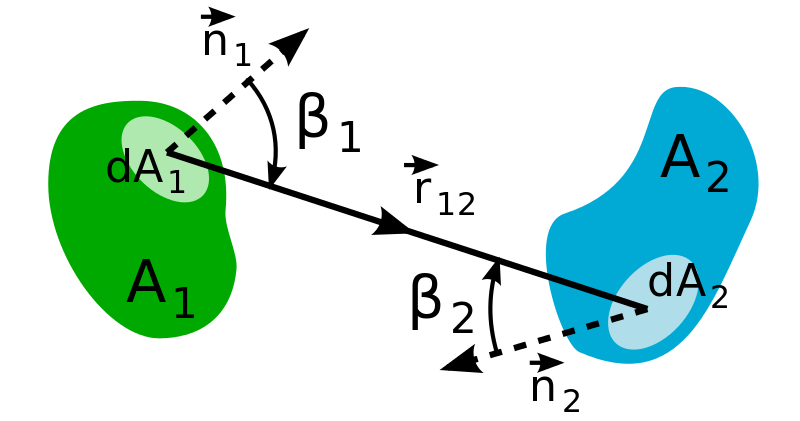
\includegraphics[width=0.75\textwidth]{images/Fotometrisches_Grundgesetz_Schema.png}
    \label{fig:shadowmap1}
      \end{figure}
  


\begin{Satz}
Die Strahlungsleistung $\phi:= \frac{ \partial Q}{\partial t}$, die von einer abstrahlenden Fläche $A_2$  auf eine Fläche $A_1$ übertragen wird, berechnet sich durch
\begin{align}
\phi = \int_{A_1} \int_{\pi_s(A_2)} L(x, \omega)\cdot \cos(\beta_1) d\omega  dA_1   \; ,
\end{align}
wobei $\theta$ der Winkel zwischen der Flächennormale am Punkt $x$ und der Richtung $\omega$ ist und $\pi_s(A_2)$ das sphärische Bild von $A_2$ ist.
\end{Satz}

\begin{figure}[H]
        \centering
         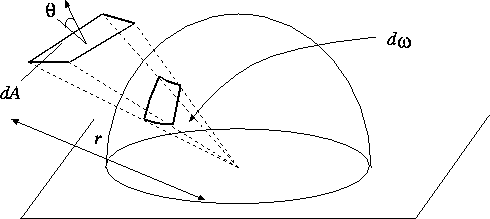
\includegraphics[width=0.75\textwidth]{images/solidangle.png}
    \label{fig:shadowmap3}
\end{figure}
Mit der Beziehung 
\begin{align}
d\omega =  \frac{1}{r^2} \cdot  \cos(\theta) dA
\end{align}     
erhalten wir die Darstellung
\begin{align}
\phi = \int_{A_1} \int_{A_2} \frac{1}{r_{12}^2}  \cdot L(x, \overline{xy}) \cdot \cos(\beta_1) \cdot \cos(\beta_2)  d A_2 dA_1 \; ,
\end{align}

\begin{Definition}
Eine Oberfläche, dessen Strahldichte für alle Punkte und Richtungen konstant ist, also
$L(x, \omega) = c$  für alle $x \in O$ und $\omega \in S^2$, bezeichnet man auch als Lambertschen Strahler. 
\end{Definition}

\begin{Definition}
Die Irradiance $E$ ist definiert durch
\begin{align}
E(x) := \int_{H^2} L_i(x, \omega) \cos{\theta} d\omega \; ,
\end{align}
also die auftreffende Strahlungsleistung pro Flächeneinheit. 
\end{Definition}

\begin{Definition}
Die Radiosity $B$ ist definiert durch
\begin{align}
B(x) := \int_{H^2} L_o(x, \omega) \cos{\theta} d\omega \; ,
\end{align}
also die ausgehende Strahlungsleistung pro Flächeneinheit. 
\end{Definition}




\begin{Definition}
Die  bidirektionale Reflektanzverteilungsfunktion (engl. Bidirectional Reflectance Distribution Function, BRDF)
ist eine Funktion $f_r (x, \omega_i, \omega_r)$, die das Reflexionsverhalten der Oberfläche eines Materials beschreibt. 
Sie hat als Eingabe die ausgehende Richtung $\omega_r$ und die eingehende Richtung  $\omega_i$ am Punkt $x$. 
Sie  liefert den Quotienten aus Strahlungsdichte und Bestrahlungsstärke für die ausgehende Richtung $\omega_r$ und die eingehende Richtung  $\omega_i$ am Punkt $x$.
Sie gibt somit die Abhängigkeit des reflektierten Lichts von der einfallenden Lichtstärke an: 
\begin{align}
\underbrace{L_r(x, \omega_r)}_{\substack{\text{Reflektierte Strahlung} \\ \text{in Richtungen $\omega_r$}}} =\underbrace{\int_{H^2} \underbrace{f_r (x, \omega, \omega_r)}_{\substack{\text{Reflektionseigenschaft} \\ \text{des Materials}}} \cdot  \underbrace{L_i(x, \omega) \cdot  \cos(\theta) }_{\substack{\text{Eingehende Strahlung} \\ \text{aus Richtung $\omega$}}} d\omega}_{\substack{\text{Summation über  alle } \\ \text{eingehenden Richtungen $\omega$}}} 
\end{align}
Letztere Gleichung wird  Reflectance-Gleichung genannt.
\end{Definition}
 \begin{figure}[H]
    \centering
    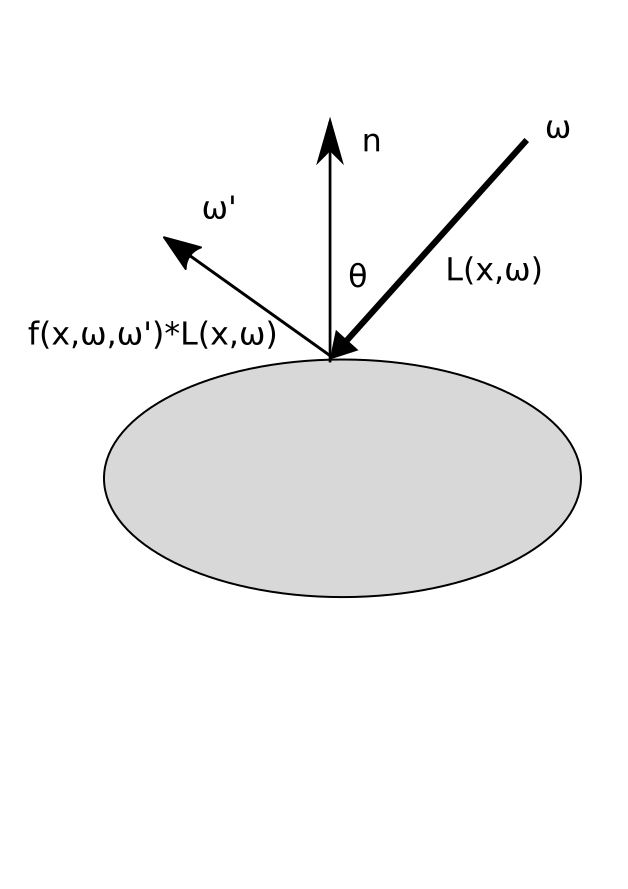
\includegraphics[width=0.75\textwidth]{images/brdf.png}
    \caption{BRDF Funktion}
    \label{fig:raytracin_brdf}
\end{figure}




\subsection{Farbwahrnehmung und Farbmodelle}
